\documentclass[12pt]{article}
\usepackage{../../template}
\author{Daniel Chua}
\title{Data Analysis Exercise}
\begin{document}
\maketitle

\section{Introduction}

Data from a nonlinear model is fitted in this data analysis exercise. The graphics file \verb|ellipses28.jpg| is analysed.

\section{Methods}

A ruler is used to measure the ellipses. It is 150 mm long with the smallest division being 1 mm. In measuring the axes, the ruler is first placed parallel to the respective side of the calibration square. While remaining parallel, it is then moved up and down to search for the greatest reading, which is recorded as the length of said axis.

The main sources of uncertainties are as follows. There is the human factor, as the ruler may not be exactly parallel to the side of the calibration square. The measured "axis" may be in fact diverge from the horizontal or vertical axes by a few degrees, which would lead to errors. The second source of error comes from the finite number of divisions. There is a smallest distance between divisions, so any measurement between divisions would be rounded to the closest mark.

In light of both sources of errors, the uncertainties of the measurements are taken to be 1 mm, the size of the smallest division. Usually, 0.5 mm, or half of the size of the smallest division is used. However, a more conservative estimate is used to account for human error.

The measurements, numbers, and scale factors can be found in \ref{rawdata}.

\section{Analysis}

Orthogonal Distance Regression is used to fit the curve. Simply put, this operates similarly to the Least Squares Method, only that the distance is taken to be the orthogonal distance between the curve and the actual data point, instead of the vertical distance. Monte Carlo methods are used to account for systematic uncertainties from the calibration squared. The code takes into account systematic errors from calibration, and measurement errors are assumed to come from a gaussian distribution. Values for each fit are in table \ref{values}, and the fits for Gaussian, Lognormal and Laplacian curves are as follows. Note that "quasi $\chi^2$" is a value that converges to $\chi^2$ as uncertainties go to 0. Since uncertainties are relatively low, we take that to be the $\chi^2$ value in the analysis.

Note: the code is mostly taken from \verb|odr_fit_extended.py| found on \url{https://www.physics.utoronto.ca/apl/python/index.htm}.

\begin{center}
    \begin{table}\label{values}
    \begin{tabular}{|c||c|c|c|c|}
        \hline
        Method & $\mu$ & $y_\mu$ & $\sigma$ & Quasi $\chi^2$ \\
        \hline\hline
        Sample & $24.5 \pm 0.7$ & $60 \pm 1$ & $7.2 \pm 0.2$ & NA \\
        \hline
        Gaussian & $24.6 \pm 0.5$ & $80.1 \pm 2$ & $5.2 \pm 0.3$ & 0.677 \\
        \hline
        Lognormal & $0 \pm 3 \times 10^6$ & $2 \times 10^8$ & $9 \times 10^7$ & 78.2 \\
        \hline
        Laplacian & $24 \pm 1$ & $4 \pm 1$ & $140 \pm 80$ & 3.17 \\
        \hline
    \end{tabular}
\end{table}
\end{center}

\begin{figure}\label{gauss}
    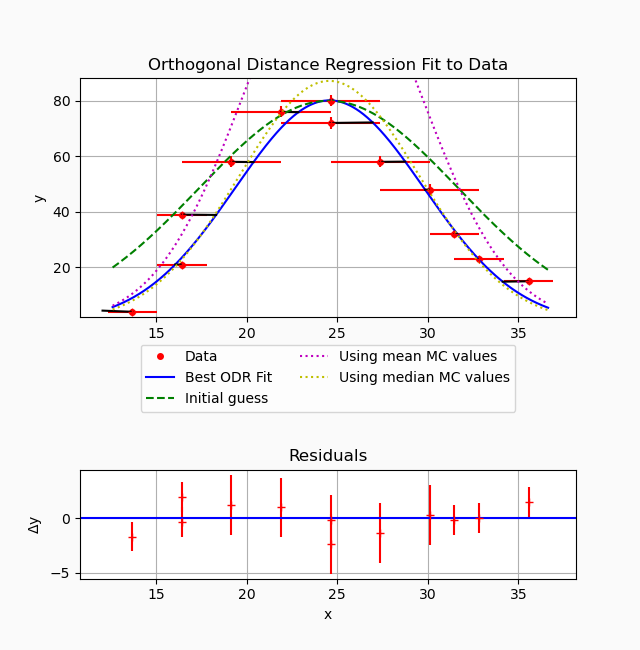
\includegraphics[width=\textwidth]{gaussian.png}
    \caption{Gaussian Fit}
\end{figure}

\begin{figure}\label{log}
    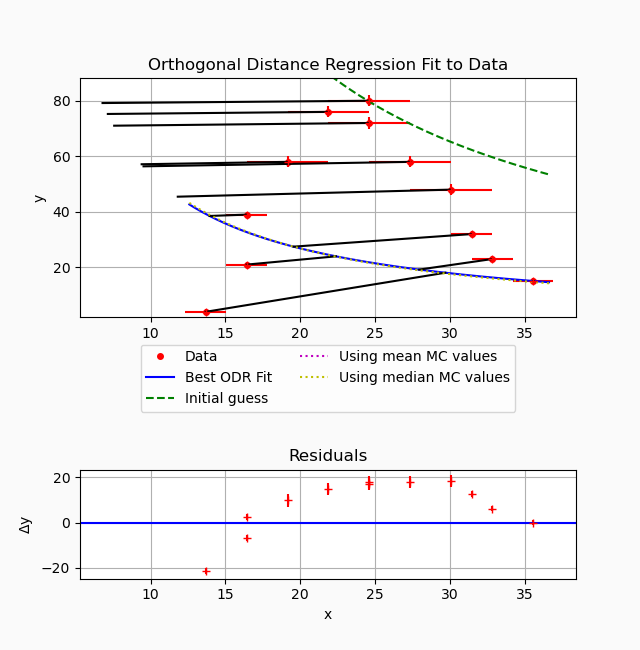
\includegraphics[width=\textwidth]{lognormal.png}
    \caption{Lognormal Fit}
\end{figure}

\begin{figure}\label{lap}
    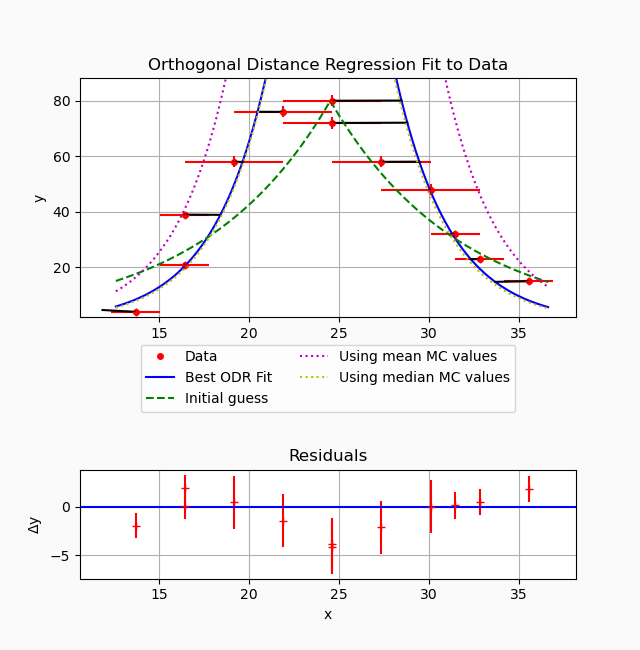
\includegraphics[width=\textwidth]{laplacian.png}
    \caption{Laplacian Fit}
\end{figure}

In the table, "sample" denotes the sample means and standard deviations used as the initial guesses for the code. Equations for the uncertainties can be found in \ref{math}.

\section{Discussion}

Based on the graphs, it is visually obvious that the correct fit is Gaussian, because the produced curve fits the shape of the data, and there is no observable patterns in the residuals, with most data points lying on the fit within uncertainties. To further support this, note that it has the lowest uncertainties, a $\chi^2$ valued closed to 1, and that its means and standard deviation in the fit are closest to the sample values. The best estimates are extracted here for convenience

$$\mu = 24.6 \pm 0.5, y_\mu = 80.1 \pm 2, \sigma = 5.2 \pm 0.3, \chi^2 = 0.677$$

\subsection{$\mu$}

For the measurements along the horizontal axis, since the uncertainty for the predicted value of $\mu$ is low, and is close to the sample value, there is no reason to suggest that the estimated measurement uncertainties are either too large or too small.

\subsection{$y_\mu$}\label{excuse}

There is an issue with the measurements along the vertical axis. $y_\mu$ according to the fit and sample $y_\mu$ have a non-negligible difference. This cannot be explained by measurement uncertainties, since the values for the horizontal axis are generally lower, hence with greater relative uncertainties, yet the relative uncertainty for $\mu$ is low, and both predicted $\mu$ and sample $\mu$ are equal within uncertainties. While it is theoretically possible for there to be systematic error in measuring the vertical axis only, it is unlikely that it does not affect the measurements for the horizontal axis. Moreover, measurements were repeated without significant changes. It is hypothesised that this could be due to printing quality. The measured "height" of the ellipses highly depend on the visibility of its top and bottom edges, which is less of a concern for its width. Poor printing quality or poor eyesight could obscure where the shape ends, which could systematically reduce the measured values of $y$. The fact that sample $y_\mu$ is lower supports this.

\subsection{$\sigma$}

The sample and predicted values for standard deviation are not equal even when accounting for uncertainties. The reasons for this cannot be entirely explained by the measurements along the horizontal axis, since given the good fit for $\mu$, the only possible explanation is that somehow all the bigger measurements are enlarged, and vice versa. It is more likely that this is an artifact of poor measurements along the vertical axis, as explained above, which required $\sigma$ to deviate from its original value to produce a better fit.

\subsection{Comments}

If there were more time, I would print out the sheet with a higher quality using darker ink, to make sure the shape is more clear and avoid the systematic errors as described in \ref{excuse}. I would also use a caliper to measure the ellipses, which would lead to a lower uncertainty. However, this would also worsen another source of error, where the measured line is not exactly the horizontal or vertical axis.

\appendix


\section{Uncertainty Calculations} \label{math}

Let $x$ and $y$ denote horizontal and vertical measurements, $c$ the length of the calibration square, and $x'$ the adjusted length in units. $\mu$ and $y_\mu$ denote the means for $x$ and $y$ respectively, and there are $n$ terms of each. $\sigma$ is the standard deviation of $x$. All of these are prepended with $\Delta$ to denote their uncertainties. We use the convention

\begin{equation}
    \Delta f(x_1,\dots,x_n) = \sqrt{\sum_i \left(\Delta x_i \del{f}{x_i}\right)^2}
\end{equation}

Then

\begin{equation}
    \Delta x' = \sqrt{(x\Delta c)^2 + (c\Delta x)^2}
\end{equation}

\begin{equation}
    \Delta \mu = \frac{\sqrt{\sum_i \Delta x'^2_i}}{n}
\end{equation}

and the same holds for $y'$ and $y_\mu$.

\begin{equation}
    \Delta \sigma = \frac{\sum_i 2(x'_i - \mu)\sqrt{\Delta x'^2_i + \Delta \mu^2}}{2(n-1)\sigma}
\end{equation}

\section{Raw Data}\label{rawdata}

\begin{table}[h!]
\begin{tabular}{| c | c | c | c |}
\hline
$n$ & $s$ & $x$ (mm)  & $y$ (mm) \\
\hline \hline
1 & 1 & 10 & 4 \\
\hline
2 & 1 & 12 & 21 \\
\hline
3 & 2 & 8 & 38 \\
\hline
4 & 1 & 26 & 15 \\
\hline
5 & 1 & 18 & 32 \\
\hline
6 & 1 & 24 & 23 \\
\hline
7 & 2 & 7 & 29 \\
\hline
8 & 2 & 9 & 36 \\
\hline
9 & 2 & 10 & 29 \\
\hline
10 & 2 & 11 & 24 \\
\hline
11 & 1 & 12 & 39 \\
\hline
12 & 2 & 9 & 40 \\
\hline
\end{tabular}
\end{table}

\end{document}
